% chap10sec09

\section{Vector analysis}

We conclude this chapter with a few applications of the preceding material to theorems concerning vector analysis in $\R^3$. 
These are special cases of theorems about differential forms, but are usually stated in different terminology. 
We are thus faced with the job of translating from one language to another.

\begin{mydef}
    \myKeyword{Vector fileds}

\end{mydef}

\begin{thm}
    \label{thm:10.43}
    Suppose $E$ is an open set in $\R^3$, $u \in \mathscr{C}''(E)$, and $\mathbf{G}$ is a vector field in $E$, of class $\mathscr{C}''$.
    \begin{enumerate}[(a)]
        \item If $\mathbf{F} = \mathbf{n}abla u$, then $\mathbf{n}abla \times \mathbf{F} = \mathbf{0}$.
        \item If $\mathbf{F} = \mathbf{n}abla \times \mathbf{G}$, then $\mathbf{n}abla \cdot \mathbf{F} = 0$.
    \end{enumerate}

    Furthermore, if $E$ is $\mathscr{C}''$-equivalent to a convex set, 
    then (a) and (b) have converses, 
    in which we assume that $\mathbf{F}$ is a vector field in $E$, of class $\mathscr{C}'$:
    \begin{enumerate}[(a')]
        \item If $\mathbf{n}abla \cdot \mathbf{F} = \mathbf{0}$, then $\mathbf{F} = \mathbf{n}abla u$ for some $u \in \mathscr{C}''(E)$.
        \item If $\mathbf{n}abla \times \mathbf{F} = 0$, then $\mathbf{F} = \mathbf{n}abla \times \mathbf{G}$ for some vector field $\mathscr{G}$. in $E$, of class $\mathscr{C}''$
    \end{enumerate}
\end{thm}

\begin{mydef}
    \label{mydef:10.44}
    \myKeyword{Volume elements}
    The $k$-form 
    \begin{equation*}
        \d x_1 \wedge \cdots \wedge \d x_k
    \end{equation*}
    is called the volume element in $\R^k$.
    It is often denoted by $\d V$
    (or by $\d V_k$ if it seems desirable to indicate the dimension explicitly),
    and the notation 
    \begin{equation}
        \label{eq:10.126}
        \int_{\Phi} f(\mathbf{x}) 
        \d x_1 \wedge \cdots \wedge \d x_k
        = \int_{\Phi} f \d V
    \end{equation}
    is used when $\Phi$ is a positively oriented $k$-surface in $\R^k$ and $f$ is a continuous function on the range of $\Phi$.

    The reason for using this terminology is very simple: 
    If $D$ is a parameter domain in $\R^k$, 
    and if $\Phi$ is a 1-1 $\mathscr{C}'$-mapping of $D$ into $\R^k$, 
    with positive Jacobian $J_{\Phi}$, then the left side of \eqref{eq:10.126} is
    \begin{equation*}
        \int_D f (\Phi(\mathbf{u})) J_{\Phi}(\mathbf{u}) \d \mathbf{u} =
        \int_{\Phi(D)} f(\mathbf{x}) \d \mathbf{x},
    \end{equation*}
    by \eqref{eq:10.35} and Theorem \ref{thm:10.9}.
\end{mydef}

In particular, when $f= 1$, \eqref{eq:10.126} defines the volume of $\Phi$. 
We already saw a special case of this in \eqref{eq:10.36}.
The usual notation for $\d V_2$ is $\d A$.

\begin{mydef}
    \label{mydef:10.45}
    \myKeyword{Green's theorem}
    Suppose $E$ is an open set in $\R^2$, $\alpha \in  \mathscr{C}'(E)$, $\beta \in  \mathscr{C}'(E)$,
    and $Q$ is a closed subset of $E$, with positively oriented boundary $\partial \Omega$, as described
    in Sec. \ref{mydef:10.31}. Then
    \begin{equation}
        \label{eq:10.127}
        \int_{\partial \Omega} \left( 
            \alpha \d x + \beta \d y 
            \right) = 
        \int_{\Omega} \left( 
            \frac{\partial \beta}{\partial x} -
            \frac{\partial \alpha}{\partial y} 
            \right) \d A .
    \end{equation}
\end{mydef}

% todo add proof
\begin{equation}
    \label{eq:10.128}
    \frac{1}{2} \int_{\partial \Omega}
    \left( x \d y - y \d x \right) = 
    A(\Omega) ,
\end{equation}
the area of $\Omega$.

\begin{mydef}
    \label{mydef:10.46}
    \myKeyword{Area elements in $\R^3$}
    Let $\Phi$ be a 2-surface in $\R^3$, of class $\mathscr{C}'$, 
    with parameter domain $D \subset \R^2$. 
    Associate with each point $(u, v) \in D$ the vector
    \begin{equation}
        \label{eq:10.129}
        \mathbf{N}(u,v) = 
        \frac{\partial (y,z)}{\partial (u,v)} \mathbf{e}_1 + 
        \frac{\partial (z,x)}{\partial (u,v)} \mathbf{e}_2 + 
        \frac{\partial (x,y)}{\partial (u,v)} \mathbf{e}_3 .
    \end{equation}
    The Jacobians in \eqref{eq:10.129} correspond to the equation
    \begin{equation}
        \label{eq:10.130}
        (x,y,z) = \Phi(u,v).
    \end{equation}
    If $f$ is a continuous function on $\Phi(D)$, 
    the \myKeywordblue{area integral} of $f$ over $\Phi$ is defined to be
    \begin{equation}
        \label{eq:10.131}
        \int_{\Phi} f \d A = 
        \int_D f(\Phi(u,v)) \left| \mathbf{N}(u,v) \right| \d u \d v.
    \end{equation}
    In particular, when $f= 1$ we obtain the \myKeywordblue{area} of $\Phi$, namely,
    \begin{equation}
        \label{eq:10.132}
        A(\Phi) = \int_{D} \left| \mathbf{N}(u,v) \right| \d u \d v. 
    \end{equation}
    The following discussion will show that (\eqref{eq:10.131}) and its special case (\eqref{eq:10.132}) are reasonable definitions. 
    It will also describe the geometric features of the vector $\mathbf{N}$.

    Write $\Phi = 
    \phi_1 \mathbf{e}_1 + 
    \phi_2 \mathbf{e}_2 + 
    \phi_3 \mathbf{e}_3 $ ,
    fix a point $\mathbf{p}_0 = (u_0,u_0) \in D$, 
    put $\mathbf{N} = \mathbf{N}(\mathbf{p}_0)$, put 
    \begin{equation}
        \label{eq:10.133}
        \alpha_i = (D_1 \phi_i)(\mathbf{p}_0), \quad 
        \beta_i  = (D_2 \phi_i)(\mathbf{p}_0)  \quad 
        (i = 1,2,3)
    \end{equation}
    and let $T \in L(\R^2, \R^3)$ be the linear transformation given by
    \begin{equation}
        \label{eq:10.134}
        T(u,v) = \sum_{i=1}^{3}\left( \alpha_i u + \beta_i v \right)\mathbf{e}_i .
    \end{equation}
    Note that $T = \Phi'(\mathbf{p}_0)$, in accordance with Definition \ref{mydef:9.11}.

    Let us now assume that the rank of $T$ is 2. 
    (If it is 1 or 0, then $\mathbf{N} = \mathbf{0}$, 
    and the tangent plane mentioned below degenerates to a line or to a point.) 
    The range of the affine mapping
    \begin{equation}
        (u,v) \rightarrow \Phi(\mathbf{p}_0) + T(u,v)
    \end{equation}
    is then a plane $\prod$, called the \myKeywordblue{tangent plane} to $\Phi$ at $\mathbf{p}_0$ . 
    [One would like to call $\prod$ the tangent plane at $\Phi(\mathbf{p}_0)$, rather than at $\mathbf{p}_0$ ; 
    if $\Phi$ is not one-to-one, this runs into difficulties.]
    If we use \eqref{eq:10.133} in \eqref{eq:10.129}, we obtain
    \begin{equation}
        \label{eq:10.135}
        \mathbf{N} = 
        \left( \alpha_2 \beta_3 - \alpha_3 \beta_2 \right) \mathbf{e}_1 +
        \left( \alpha_3 \beta_1 - \alpha_1 \beta_3 \right) \mathbf{e}_2 +
        \left( \alpha_1 \beta_2 - \alpha_2 \beta_1 \right) \mathbf{e}_3 ,
    \end{equation}
    and \eqref{eq:10.134} shows that 
    \begin{equation}
        \label{eq:10.136}
        T \mathbf{e}_1 = \sum_{i=1}^{3} \alpha_i \mathbf{e}_i ,
        \quad 
        T \mathbf{e}_2 = \sum_{i=1}^{3} \beta_i \mathbf{e}_i .
    \end{equation}
    A straightforward computation now leads to
    \begin{equation}
        \label{eq:10.137}
        \mathbf{N}\cdot (T \mathbf{e}_1) = 0 =
        \mathbf{N}\cdot (T \mathbf{e}_2) .
    \end{equation}
    Hence $\mathbf{N}$ is perpendicular to $\prod$. 
    It is therefore called \myKeywordblue{the normal to $\Phi$ at $\mathbf{p}_0$} .

    A second property of $\mathbf{N}$, also verified by a direct computation based on \eqref{eq:10.135} and \eqref{eq:10.136}, is that the determinant of the linear transformation of $\R^3$ that takes $\{e_1, e_2 , e_3\}$ to $\{T\mathbf{e}_1, T\mathbf{e}_2 , \mathbf{N}\}$ is $\left\| \mathbf{N} \right\|^2 0$ (Exercise \ref{ex:10.30}). The 3-simplex
    \begin{equation}
        \label{eq:10.138}
        \left\{ \mathbf{0}, T\mathbf{e}_1, T\mathbf{e}_2, \mathbf{N} \right\}
    \end{equation}
    is thus \myKeywordblue{positively oriented}.

    The third property of $\mathbf{N}$ that we shall use is a consequence of the first two:
    The above-mentioned determinant, whose value is $|\mathbf{N}|^2$, is the volume of the parallelepiped with edges $[\mathbf{0}, T\mathbf{e}_1]$, $[\mathbf{0}, T\mathbf{e}_2]$, $[\mathbf{0}, \mathbf{N}]$. 
    By \eqref{eq:10.137}, $[\mathbf{0}, \mathbf{N}]$ is perpendicular to the other two edges. 
    \myKeywordblue{The area of the parallelogram with vertices}
    \begin{equation}
        \label{eq:10.139}
        \mathbf{0}, 
        T \mathbf{e}_1 ,
        T \mathbf{e}_2 ,
        T (\mathbf{e}_1 + \mathbf{e}_2)
    \end{equation}
    \myKeywordblue{is therefore $\left| \mathbf{N} \right|$}.

    This parallelogram is the image under $T$ of the unit square in $\R^2$. 
    If $E$ is any rectangle in $\R^2$ , it follows 
    (by the linearity of $T$) that the area of the
    parallelogram $T(E)$ is
    \begin{equation}
        \label{eq:10.140}
        A(T(E)) = \left| \mathbf{N} \right| A(E) =
        \int_E \left| \mathbf{N}(u_0,v_0) \right| \d u \d v .
    \end{equation}
    We conclude that \eqref{eq:10.132} is correct when $\Phi$ is affine. 
    To justify the definition \eqref{eq:10.132} in the general case, divide $D$ into small rectangles, pick a point $(u_0, v_0)$ in each, and replace $\Phi$ in each rectangle by the corresponding tangent plane. 
    The sum of the areas of the resulting parallelograms, obtained via \eqref{eq:10.140}, is then an approximation to $A(\Phi)$. 
    Finally, one can justify \eqref{eq:10.131} from \eqref{eq:10.132} by approximating $f$ by step functions.
\end{mydef}

\begin{newexample}
    \label{newexample:10.47}
    Let $0 <a< b$ be fixed. Let $K$ be the 3-cell determined by
    \begin{equation*}
        0 \leq t \leq a , \quad
        0 \leq u \leq 2\pi , \quad
        0 \leq v \leq 2\pi
    \end{equation*}
    The equations
    \begin{equation}
        \label{eq:10.141}
        \begin{array}{l}
            x = t \cos u \\
            y = (b + t \sin u) \cos v \\
            z = (b + t \sin u) \sin v \\
        \end{array}
    \end{equation}
    describe a mapping $\Psi$ of $\R^3$ into $\R^3$ which is 1-1 in the interior of $K$, such that $\Psi(K)$ is a solid torus. Its Jacobian is
    \begin{equation*}
        J_{\Psi} = \frac{\partial(x,y,z)}{\partial(t,u,v)} = t(b+t\sin u)
    \end{equation*}
    which is positive on $K$, except on the face $t = 0$. 
    If we integrate $J_{\Psi}$ over $K$, we obtain
    \begin{equation*}
        \operatorname{vol}(\Psi(K)) = 2 \pi^2 a^2 b
    \end{equation*}
    as the volume of our solid torus.

    Now consider the 2-chain $\Phi = \partial \Psi$. 
    (See Exercise \ref{ex:10.19}.) 
    $\Psi$ maps the faces $u = 0$ and $u = 2\pi$ of $K$ onto the same cylindrical strip, but with opposite orientations. 
    $\Psi$ maps the faces $v = 0$ and $v = 2\pi$ onto the same circular disc, but with opposite orientations.
    $\Psi$ maps the face $t = 0$ onto a circle, which contributes 0 to the 2-chain $\partial \Psi$. 
    (The relevant Jacobians are 0.) 
    Thus $\Phi$ is simply the 2-surface obtained by setting $t = a$ in \eqref{eq:10.141}, with parameter domain $D$ the square defined by $0 \leq u \leq 2\pi, 0 \leq v \leq 2\pi$.

    According to \eqref{eq:10.129} and \eqref{eq:10.141}, 
    the normal to $\Phi$ at $(u, v) \in D$ is thus the vector
    \begin{equation*}
        \mathbf{N}(u,v) = a(b+a\sin u) \mathbf{n}(u,v)
    \end{equation*}
    where 
    \begin{equation*}
        \mathbf{n}(u,v) = 
        (\cos u) \mathbf{e}_1 + 
        (\sin u \cos v) \mathbf{e}_2 + 
        (\sin u \sin v) \mathbf{e}_3 . 
    \end{equation*}
    Since $|\mathbf{n}(u, v)| = 1$, 
    we have $|\mathbf{N}(u, v)| = a(b + a \sin u)$, 
    and if we integrate this over $D$, \eqref{eq:10.131} gives
    \begin{equation*}
        A(\Phi) = 4\pi^2 ab
    \end{equation*}
    as the surface area of our torus.
    \begin{figure}[htbp]
        \centering
        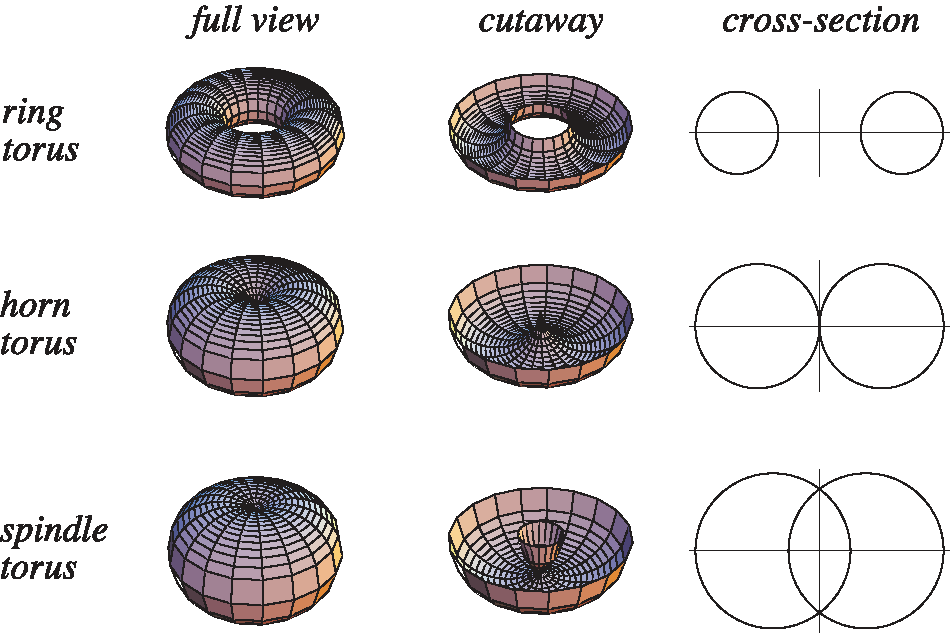
\includegraphics[width=0.7\linewidth]{pic/StandardTori701.pdf}
        \caption{StandardTori701}
        \label{fig:StandardTori701}
    \end{figure}
    If we think of $\mathbf{N} = \mathbf{N}(u, v)$ as a directed line segment, 
    pointing from $\Phi(u, v)$ to $\Phi(u, v) + \mathbf{N}(u, v)$, 
    then $\mathbf{N}$ points outward, 
    that is to say, away from $\Psi(K)$. 
    This is so because $\mathbf{J}_{\Psi} > 0$ when $t = a$.

    For example, take $u = v = \pi/2$, $t = a$. 
    This gives the largest value of $z$ on $\Psi(K)$, 
    and $\mathbf{N} = a(b + a)\mathbf{e}_3$ points ``upward'' for this choice of $(u, v)$.
\end{newexample}

\begin{mydef}
    \label{mydef:10.48}
    \myKeyword{Integrals of 1-forms in $\R^3$}
    
\end{mydef}

\begin{mydef}
    \label{mydef:10.49}
    \myKeyword{Integrals of 2-forms in $\R^3$}
    
\end{mydef}

\begin{mydef}
    \label{mydef:10.50}
    \myKeyword{Stokes' formula}
    
    \begin{equation}
        \label{eq:10.145}
        \int_{\Phi} \left( \mathbf{n}abla \times \mathbf{F} \right) \cdot \mathbf{n} \d A = 
        \int_{\partial \Phi} \left( \mathbf{F \cdot t} \right)  \d s
    \end{equation}
\end{mydef}

\begin{mydef}
    \label{mydef:10.51}
    \myKeyword{The divergence theorem}
    
\end{mydef}

